\section{Introduction}

COACHES project aims at developing a prototype robotic system for user assistance in a shopping mall.
The COACHES robots will use different modalities, i.e., speech and displayed information,
to interact with the mall visitors, shopkeepers and mall managers.
The scenario where the COACHES robots and systems will be deployed is provided
by a mall called ``Rive de l’orne'', located in the city of Caen, France.

A set of use cases will be implemented to show the feasibility of the approach and to assess the effectiveness of the proposed solutions with actual users.
In particular, this document contains:
\begin{enumerate}
\item A brief description of the test facilities;
\item A set of uses cases that focus on two main components of the entire system,
namely short-term human-robot interaction and safe navigation.
\end{enumerate}

\section{Test facilities: Collaboration with the Mall Rives de l'Orne}
The test facilities concerns the Mall Rives de l'Orne. Ç Rive de lÕorne È is a new and modern mall at Caen city (France). It is composed of two face-to-face buildings separated by a large main square. At the first floor of the two buildings, there are many shops and restaurants. In the main square, there is a cinema. This space is surrounded by tramway stations and a train station. This mall is visited by more than 100,000 customers every year. In addition to that, several elderly people live in the new apartments at the other floors of the buildings. These people have their habit and there are frequent customers of the mall \ref{mall}. Two meetings have been organized ($23^{th}$ October and $12^{th}$ December 2014)to define the equipments to install in terms of cameras and sensors (RFID) to send some information to robots about shops, the planning of the robot deployment in the mall and some local dissemination actions. A visit of all partners have been organized during the kickoff meeting. 

\begin{figure}[!t]
\begin{center}
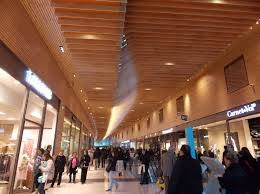
\includegraphics[width=0.42\linewidth]{InsideRivedelOrne}
\caption{Inside the mall}
\label{mall}
\end{center}
\end{figure}

\begin{figure}[!t]
\begin{center}
\includegraphics[width=0.7\linewidth]{MapsRorne}
\caption{The map}
\label{default}
\end{center}
\end{figure}


\section{Use cases for short-term interaction and navigation}

COACHES project envisages the implementation of a set of use cases
to show the feasibility of the approach and to assess the effectiveness
of the proposed solutions with actual users.
To this end, different use cases will be implemented, focusing on two main
components of the entire system:
\begin{enumerate}
\item Short-term human-robot interaction;
\item Safe navigation.
\end{enumerate}


\subsection{Customer asks for help carrying his/her bag}

The robot is called by a manager (or by the customer himself) to assist
someone in carrying his/her bag. The robot must reach
the exit of the shop and approach the dedicated loading area. When
in position he looks for the customer and as soon as he establishes
contact, he asks the user to load the bag in the appropriate container.
Once loaded, the robot will ask the customer if he is in a hurry.
If the customer is in a hurry, the robot will proceed at a sustained
speed to the parking lot. In the other case, the robot will leisurely
proceed to the parking lot, proposing intermediate stops to shops
with interesting discounts.



\subsection{Proposing an ice cream to a child}

Manager from local ice cream shop asks robot to inform children about
a special discount. The robot looks around for children. When it detects
one, it approaches him and informs him and his parents of the discount. The child
is passionate about having an ice cream; but before directing him
there, the robot asks for the parent's authorization. Once the parents
agree to allow the child to follow the robot, the robot will proceed
to the ice cream shop. 


\subsection{Customer refuses first robot proposal, accepts specific one}

Managers have told the robot that he needs to promote a special discount
for a movie. The robot is also aware, in his persistent KB, of the
existence of other secondary discounts. Since there are no people
moving around the robot starts waiting and scanning. As soon as it
sees a suitable user (at the right distance and the right speed),
the robot intercepts the customer and asks him/her if he would be interested
in the special discount for the movie. The user answers that s/he is not interested.
The robot then asks the user to slide his customer card in order to
propose the most appropriate available discount. After reading the
card, the robot finds out that the customer is a woman and that she
has made many purchases in the personal care department. 
So, the robot reasons that the special discount on the facial cream would be of interest
to her. After being informed of the discount, the customer reveals
to be interested and asks the robot for directions to reach the specific
shop. Since not many people are moving around, the robot can safely
guide the customer himself.


\subsection{Customer asks for directions in crowded environment}

The robot has the objective to inform the customers of a certain few
available discounts. The shopping mall is very crowded and, for safety
considerations, the robot decides it should not move but rather wait
for users to approach. As soon as it detects a user, standing still at
the appropriate social distance, looking at him/her, the robot initiates
conversation and announces the available offers. The user is interested
and asks for directions. Since the robot cannot safely move, it shows
the desired path on his tablet and informs the user that 20m along
the corridor s/he will find another robot for more specific information,
if needed. The human thanks the robot and goes to the next one to
receive further directions.
